
% Section: DESIGN
\section{The Distributed Auctioneer}
\label{sec:design}

We propose a framework for devising distributed 
protocols executed by the providers that correctly simulate the auctioneer.
The framework is sufficiently general to simulate different auctions.
To illustrate its applicability, we provide two implementations 
of the framework for standard and double 
bandwidth allocation auctions, respectively.
We describe the framework in two steps. First, we provide a general definition
where we do not specify the details about how to implement the simulation
of the algorithm $\A$. Then, we describe how to simulate $\A$
by leveraging parallelism to speed up its execution.


\subsection{General Framework}
The input of the framework at each provider $j$ is a vector $\vec{b}^j$
of bids submitted to $j$ and the output is either a pair $(x,\vec{p})$ containing
an allocation $x$ and a vector of payments $\vec{p}$ or the special value $\bot$.
As illustrated in Figure~\ref{fig:framework}, the framework chains the execution
of two building blocks: \emph{bid agreement} and \emph{allocator}.
Each provider $j$ inputs $\vec{b}^j$ to the bid agreement,
which outputs either a vector $\vec{b}$ or $\bot$.
In the former case, $j$ inputs $\vec{b}$ to the allocator.
If all providers follow the protocol, then the bid agreement ensures
that they all output some vector $\vec{b}$ containing all valid bids,
and the allocator ensures that they all output a pair $(x,\vec{p})$
with probability determined by $\A$.

%% FIGURE
\begin{figure}[tbp]
	\centering
	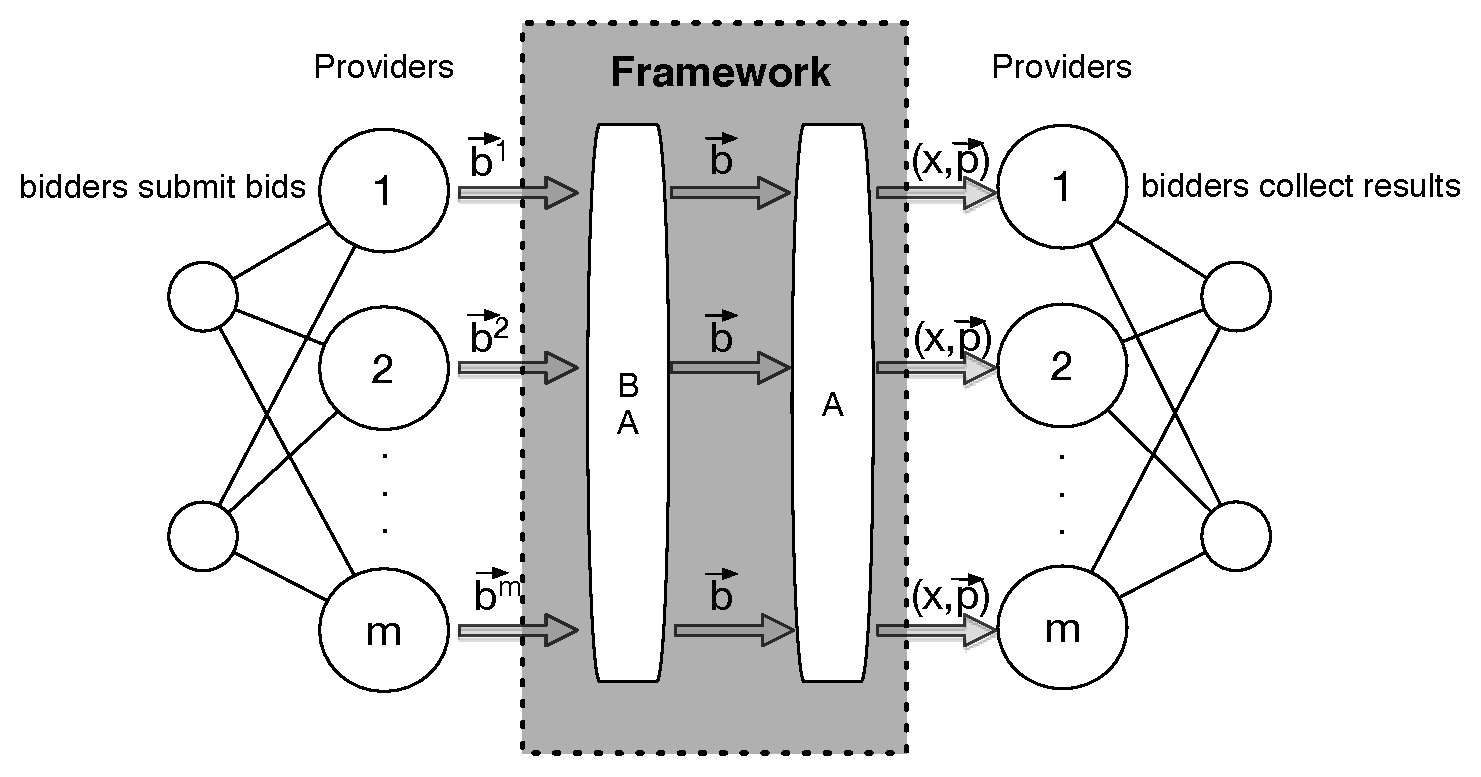
\includegraphics[width=1.0\columnwidth,keepaspectratio]{basicprotocol}
	\caption{Framework: Bid Agreement (BA) and Allocator (A)}
	\label{fig:framework}
\end{figure}

In the following paragraphs, we describe each block 
in more detail by defining properties that must be satisfied 
by any implementation of the block, and then show in the analysis that
every implementation of the framework is $k$-resilient and correctly simulates
the auctioneer based only on the properties of the blocks. This makes
the proof independent from the actual implementation.
In all blocks, an implementation $P$ must satisfy
the property of \emph{$k$-resiliency for solution preference}, i.e.,
$P$ must be a $k$-resilient equilibrium, under
the assumption that players have preference for a solution 
and number of agents not in the same coalition is sufficiently high.
Specifically, the output of every block is either some valid value or $\bot$.
We can split the set of outcomes of the block (combinations of outputs)
into the set $A$ of solutions where all providers output the same valid value
and the set $B$ of remaining outcomes. 
In a correct execution, we want the outcome to lie in $A$.
To ensure this and that the protocol is a $k$-resilient equilibrium,
we need to assume that providers obtain a higher utility for outcomes in $A$
than for outcomes in $B$ (preference for a solution), and $m > f(k)$ for
some function $f$ defined for every $k > 0$.
The assumption of preference for a solution of the framework
is equivalent to providers preferring to receive the payments.

\subsubsection*{Bid Agreement}
The input at provider $j$ is the vector $\vec{b}^j$ of bids sent to $j$.
The output is a vector $\vec{b}$ or the special value $\bot$.
In addition to $k$-resiliency for solution preference,
this block must ensure two conditions when all providers follow the protocol: 
(1) \emph{eventual agreement}, defined as
all providers eventually outputting the same vector $\vec{b}$,
and (2) \emph{validity}, defined as,
for every bidder $i$ that submits the same bid $b_i'$
to all providers, the output at every provider is $b_i = b_i'$.

\begin{property}
\label{prop:bid-agreement}
A protocol $P$ implements bid agreement if and only if it satisfies two conditions:
(1) if all providers follow $P$, then $P$ satisfies eventual agreement and validity;
and (2) $k$-resiliency for solution preference.
\end{property}

If we can assume that the bids of malicious bidders are obtained from a finite
set of values and are equally likely, then 
a suitable approach is to use the rational consensus protocol proposed in~\cite{Afek:14},
which has inputs $\{0,1\}$ and outputs in $\{0,1,\bot\}$,
and satisfies the following two properties:
(a) if all providers follow the protocol, then all providers eventually
output the same bit, which is input by some provider;
and (b) $k$-resiliency for solution preference, assuming $m > 2k$
and that the input of every provider not in the same coalition
is either the same value or is $0$ or $1$ with equal probability.
This protocol can be used to implement the bid agreement as follows.
For each bidder $i$, provider $j$ generates a stream of bits uniquely
determined from $b_i^j$ and inputs each bit to a rational consensus instance;
if some instance outputs $\bot$, then $j$ outputs $\bot$,
otherwise, $j$ converts the stream to a bid $b_i$ and outputs a bid $b_i^*$,
where $b_i^* = b_i$ if $b_i$ is valid, or $b_i^*$ is some pre-determined valid bid otherwise.
To distinguish between different instances of rational consensus,
providers may append to the messages of each instance
the identifier of each bidder and the position of each bit.
Clearly, providers only output valid bids or the value $\bot$.
By (a), if all providers follow the protocol, then
eventual agreement and validity hold, showing (1).
Condition~(2) follows directly from (b) and $m>2k$ if
the input of every provider satisfies the assumptions of (b).
To see why these assumptions are true, notice
that, for each bidder $i$, if $i$ is not malicious, 
the input of all providers not in the same coalition is $i$'s true bid,
and if $i$ is malicious, then the bid $b_i^j$ sent by $i$ to $j$ is uniformly
distributed. If the set of possible bids is the set of all integers, 
then the stream of bits obtained from $b_i^j$ is also random.
These are reasonable assumptions, 
since we expect the behavior of malicious bidders to be arbitrary.

\subsubsection*{Allocator} The input at every provider is a vector $\vec{b}$ of bids,
and the output is either a pair $(x,\vec{p})$ or $\bot$.
We want the allocator to satisfy four conditions. First, we want the allocator
to correctly simulate $\A$, i.e., given that
all providers input the same vector $\vec{b}$ and follow the protocol,
every provider must eventually output pair $(x,\vec{p})$
with probability $\A(x,\vec{p} \mid \vec{b})$.
Second, we want resilience to collusive influences,
defined as, for all coalitions $K$ of at most $k$ elements,
if all providers not in $K$ input $\vec{b}$
and follow the protocol, then no $j \notin K$ outputs a pair $(x,\vec{p})$
with probability higher than $\A(x,\vec{p} \mid \vec{b})$,
regardless of the protocol followed by providers in $K$.
Intuitively, no coalition $K$ can influence the output of providers not in $K$,
except that they may output $\bot$ with higher probability.
Third, we want input validation to ensure that
providers have preference for solutions at the bid agreement.
More precisely, if two providers input different vectors
and follow the protocol, then they both output $\bot$,
regardless of the protocol followed by other providers.
Finally, we want $k$-resilience for solution preference
given that all providers have the same input.

\begin{property}
\label{prop:allocator}
A protocol $P$ implements the allocator if and only if it satisfies four conditions:
(1) correct simulation of $\A$; (2) resilience to collusive influence;
(3) input validation; and (4) $k$-resiliency for solution preference
if all providers have the same input.
\end{property}

We discuss implementations of the allocator in Section~\ref{sec:implementation}.

\subsubsection*{Analysis} We show in Theorem~\ref{theorem:simulation}
that a protocol that implements our framework correctly
simulates the auctioneer and is $k$-resilient.
The proof is in Appendix~\ref{app:simulation}.
%The proof appears in the full paper.

\begin{theorem}
\label{theorem:simulation}
For every protocol $P$ that implements the framework,
$P$ correctly simulates the auctioneer,
and there exists a function $f$ such that, if $m > f(k)$,
then $P$ is a $k$-resilient equilibrium.
\end{theorem}

\subsection{Parallel Allocator Framework}
\label{sec:implementation}

We describe a framework for implementations of
the allocator that satisfy Property~\ref{prop:allocator}.
We explore the possibility of parallelising the execution of $\A$ in multiple providers.
Although this approach introduces the overhead of communication between providers,
since $\A$ is often computationally intensive,
its parallelisation compensates for this overhead.

The framework consists in an initial invocation of a 
building block for \emph{input validation} followed
by the simulation of $\A$, which invokes two additional building blocks:
\emph{data transfer} and \emph{common coin}.
The input is a vector of bids and the output is either $\bot$ or a pair $(x,\vec{p})$.
At the invocation of each block, providers either output a valid value
or $\bot$; in the latter case, they output $\bot$ at the allocator.
To describe the simulation of $\A$,
it is useful to characterise the execution of $\A$
in terms of a graph of tasks, where nodes correspond to
tasks to be executed in sequence and edges 
represent data dependencies. This graph establishes a partial order
of tasks; every two tasks that are not ordered can be executed in parallel
by different providers. Figure~\ref{fig:taskdecomposition}
gives an example of a graph of $4$ tasks,
where tasks T2.1 and T2.2 can be executed in parallel.
To cope with collusion, each task $T$ is assigned to a set $S$ of at least $k+1$ providers.
If a task $T'$ is to be executed by a set $O \neq S$ of providers and $T'$ depends on
the result of $T$, then the providers of $S$ transfer data to the providers of $O$
using the data transfer building block. In a correct simulation of $\A$,
there must be one final task that depends on all other tasks,
where all providers gather all the required data to produce the final output.
Whenever providers need a random number distributed according to a 
probability distribution $\Pi$, they invoke the common coin with input $\Pi$.
Figure~\ref{fig:parallel-allocator} illustrates the framework
for the task decomposition of Figure~\ref{fig:taskdecomposition}.

%% FIGURE
\begin{figure}[tbp]
	\centering
	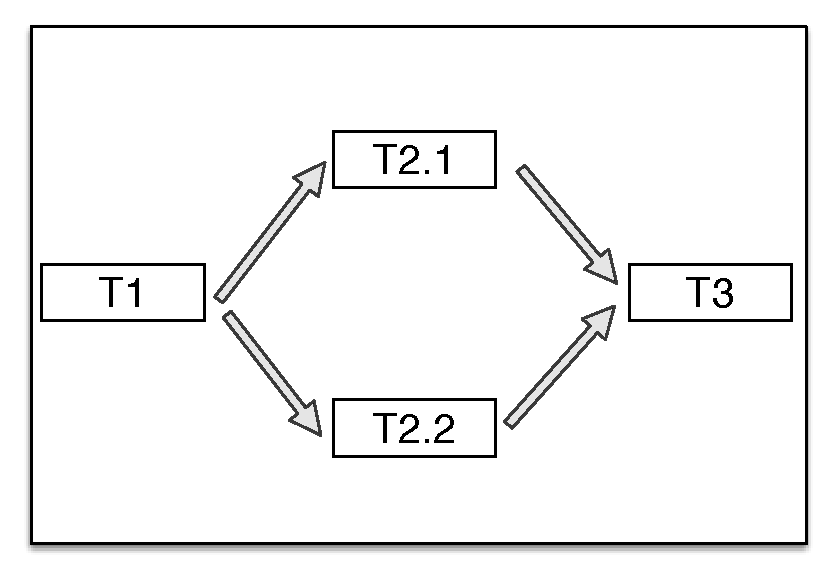
\includegraphics[width=0.85\columnwidth,keepaspectratio]{taskdecomposition}
	\caption{Decomposition of the Allocator into Tasks}
	\label{fig:taskdecomposition}
\end{figure}

As in the previous section, we describe properties that must be satisfied
by the implementations of each block and then show that every implementation
of this framework satisfies Property~\ref{prop:allocator}.

\subsubsection*{Input Validation}
The input is a vector $\vec{b}$ and the output is either
$\bot$ or $\vec{b}$. We want an implementation to satisfy 
$k$-resiliency for solution preference and that all providers 
eventually output $\vec{b}$ given that they all input $\vec{b}$,
and we need to satisfy (3) from Property~\ref{prop:allocator}.

\begin{property}
\label{prop:iv}
An implementation $P$ of the input validation must satisfy three conditions:
(1) if two providers follow $P$ and have different inputs, then they eventually output $\bot$;
(2) if all providers follow $P$ with the same input $\vec{b}$, then they eventually output $\vec{b}$;
and (3) $k$-resiliency for solution preference if all providers have the same input.
\end{property}

A simple implementation is to have providers broadcasting their vectors of bids
and outputting $\bot$ when two different vectors are detected.
This clearly satisfies (1) and (2),
whereas (3) is immediately true if providers have preference for a solution and $m > k$.

\subsubsection*{Common Coin}
The input is a probability distribution $\Pi$
and the output is either $\bot$ or a number distributed according to $\Pi$.
Given that all providers have the same input, we 
want the common coin to satisfy $k$-resilience for solution preference 
and to output the same random number.

\begin{property}
\label{prop:common-coin}
Given that all providers have input $\Pi$,
an implementation $P$ of the common coin must satisfy two conditions:
(1) if all providers follow $P$, then they eventually output 
the same value distributed according to $\Pi$;
and (2) $k$-resiliency for solution preference.
\end{property}

%% FIGURE
\begin{figure}[tbp]
	\centering
	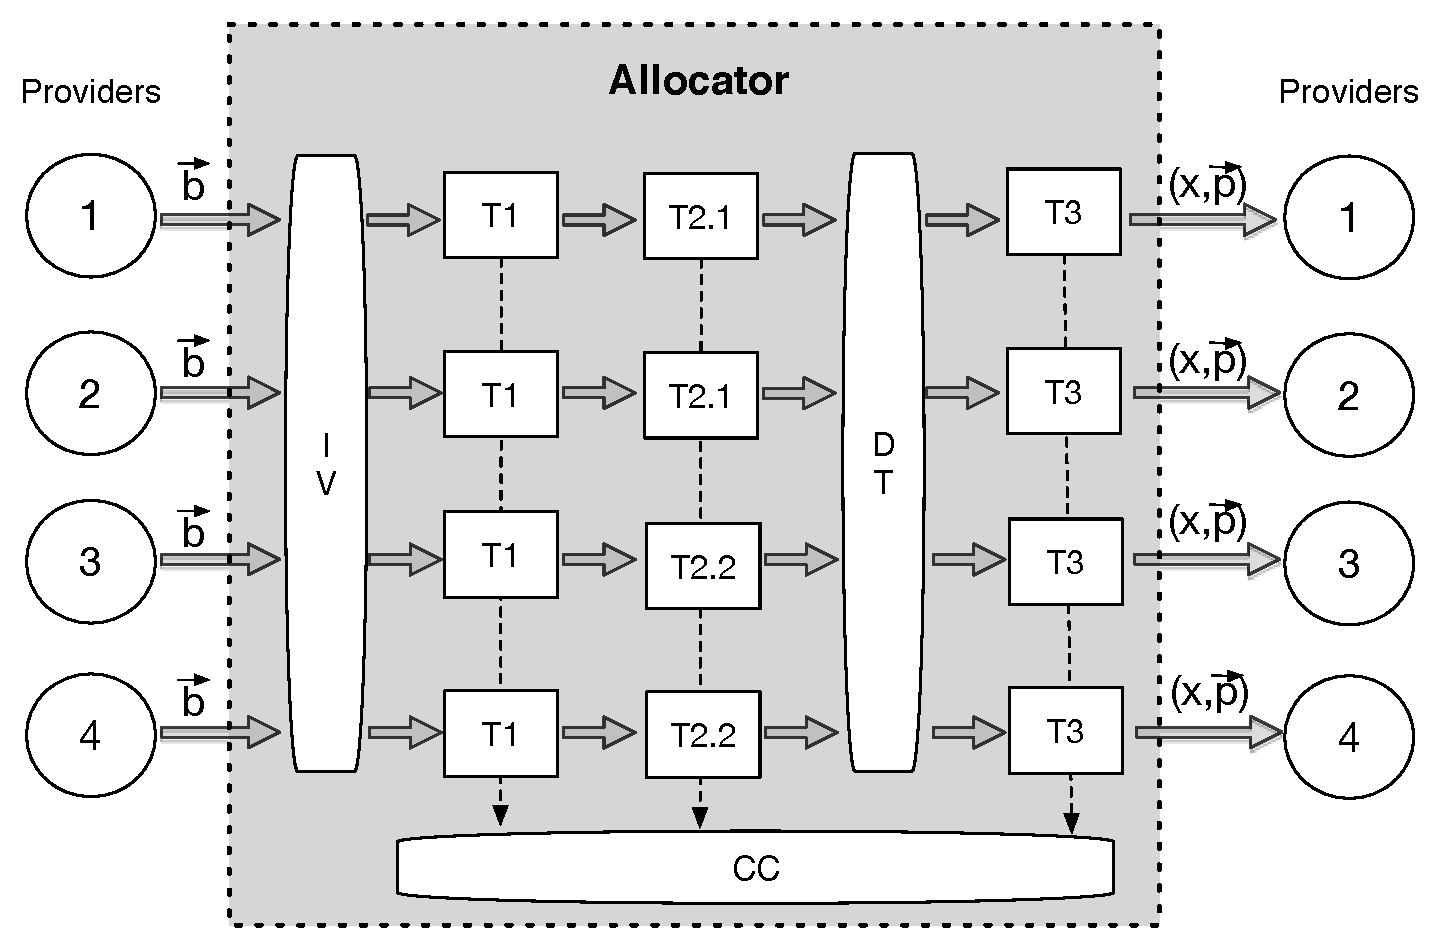
\includegraphics[width=1.0\columnwidth,keepaspectratio]{finalprotocol}
	\caption{Parallel Allocator: Input Validation (IV), Data Transfer (DT), and Common Coin (CC)}
	\label{fig:parallel-allocator}
\end{figure}

A possible implementation of the shared coin is the protocol from~\cite{Abraham:13}.
The idea is that every provider $j$ commits to a random number $r_j \in [0,1]$,
before learning the random numbers of every other provider not in its coalition.
Then, providers reveal all random numbers and compute the output by summing all numbers modulo $1$.
If some provider $j$ sees a number not in $[0,1]$ or some provider does not send
a random value compatible with its commitment, then it outputs $\bot$.
Otherwise, $j$ applies a transformation on the computed value, which is uniformly distributed in $[0,1]$,
to produce an output that is distributed according to $\Pi$.

It is clear that all providers output the same random number distributed according to the common input $\Pi$
if they follow the protocol. Assuming that $m > k$, no provider $j$ can manipulate
the probability distribution of the output by not committing to $r_j$ selected at random
without some provider outputting $\bot$, even if $j$ is in a coalition of at most $k$ providers.
Therefore, the protocol satisfies $k$-resiliency for solution preference.

\subsubsection*{Data Transfer} A set $S$ of providers inputs a value from a domain $D$.
Providers from a set $O$ either output a value from $D$ or $\bot$.
When all providers in $S$ have the same input,
we want them to output the same value in $D$ when they follow the protocol.
We only require an implementation to be $k$-resilient if $|S|,|O| > k$,
since otherwise coalitions can always manipulate the output of this block.

\begin{property}
\label{prop:data-transfer}
Given that $|S|,|O| > k$ and all providers have the same input $v$,
an implementation $P$ of the data transfer must satisfy two conditions: 
(1) if all providers follow $P$, then they eventually output $v$;
and (2) $k$-resiliency for solution preference.
\end{property}

We propose a simple $k$-resilient implementation of this block,
where providers in $S$ broadcast their input to all providers in $O$.
In the end, if some provider $j \in O$ detects two different values,
then $j$ outputs $\bot$. Given that all providers
have input $v$ and that $|S|,|O| > k$,
they eventually output $v$, and
no coalition $K$ of up to $k$ providers
can cause all providers to output $v' \notin \{v,\bot\}$.
By solution preference, no provider in $K$ gains if someone lies
about the input $v$ or omits a message.

\subsubsection*{Analysis}
Theorem~\ref{theorem:allocator} shows that every implementation
of the above framework satisfies the four conditions of Property~\ref{prop:allocator}.
The proof is in Appendix~\ref{app:allocator}.
%The proof appears in the full paper.

\begin{theorem}
\label{theorem:allocator}
Every protocol $P$ that implements the parallel allocator
satisfies Property~\ref{prop:allocator}.
\end{theorem}
